\documentclass[tikz]{standalone}
%\usetikzlibrary{...}% tikz package already loaded by 'tikz' option
\usetikzlibrary{graphs}

\def\es{edge from parent[solid]}
\def\ed{edge from parent[dashed]}
\usepackage{forest}

\begin{document}
%\begin{tikzpicture}
% \node[draw] at (-10,1) {ultimate good: };
%\end{tikzpicture}

%\begin{tikzpicture}
%  \node[draw] at (-10,1) {ultimate good: };
%\end{tikzpicture}

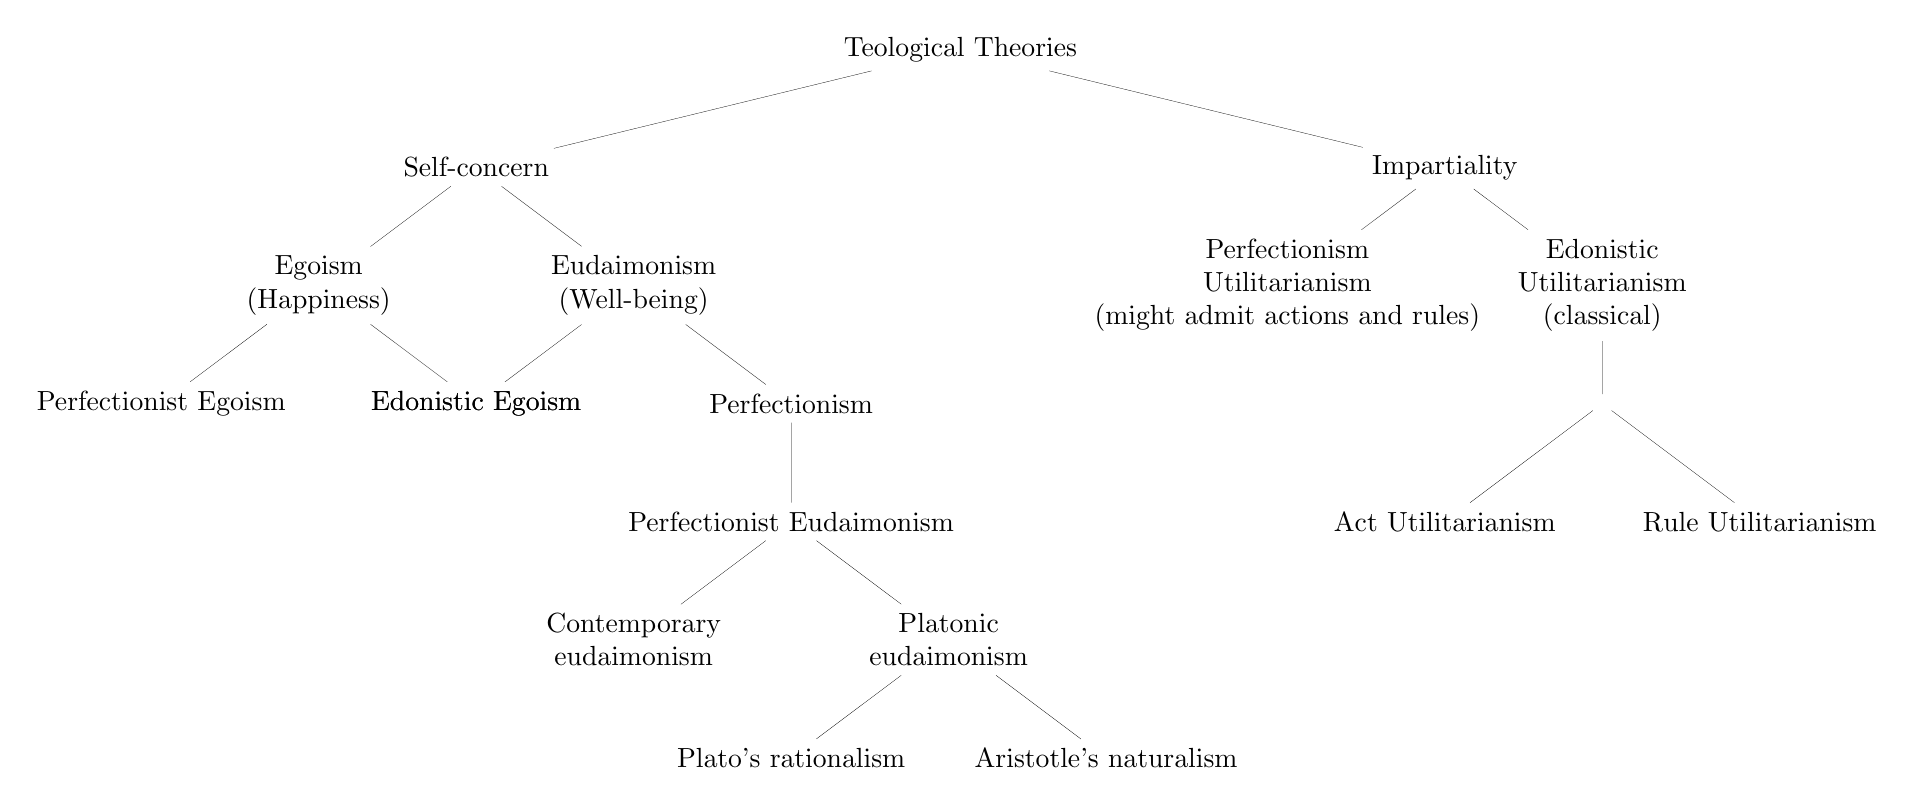
\begin{tikzpicture}[sibling distance=35em, -, ultra thin,
  every node/.style = { align=center}]]
%\footnotesize

\node {Teological Theories}
  child {node {Self-concern}
    [sibling distance=4cm]
    child {node {Egoism \\ (Happiness)}
    child {node {Perfectionist Egoism}}
    child {node {Edonistic Egoism}}
    }
    child {node (1) {Eudaimonism \\ (Well-being)}}
     [sibling distance=4cm]
    child {node {Edonistic Egoism}}
    child {node {Perfectionism}}
     [sibling distance=4cm]
    child {node {Perfectionist Eudaimonism}}
      [sibling distance=4cm]
      child {node {Contemporary\\eudaimonism}}
      child {node {Platonic\\eudaimonism}}
        [sibling distance=4cm]
        child {node {Plato's rationalism}}
        child {node {Aristotle's naturalism}}
        }
  child {node {Impartiality}
    [sibling distance=4cm]
    child {node {Perfectionism \\ Utilitarianism \\ (might admit actions and rules)}}
    child {node {Edonistic \\ Utilitarianism \\(classical)}
    child {node [] {} }
      [sibling distance=4cm]
      child {node {Act Utilitarianism}
      }
      child {node {Rule Utilitarianism}
      }
    }
  };
\end{tikzpicture}


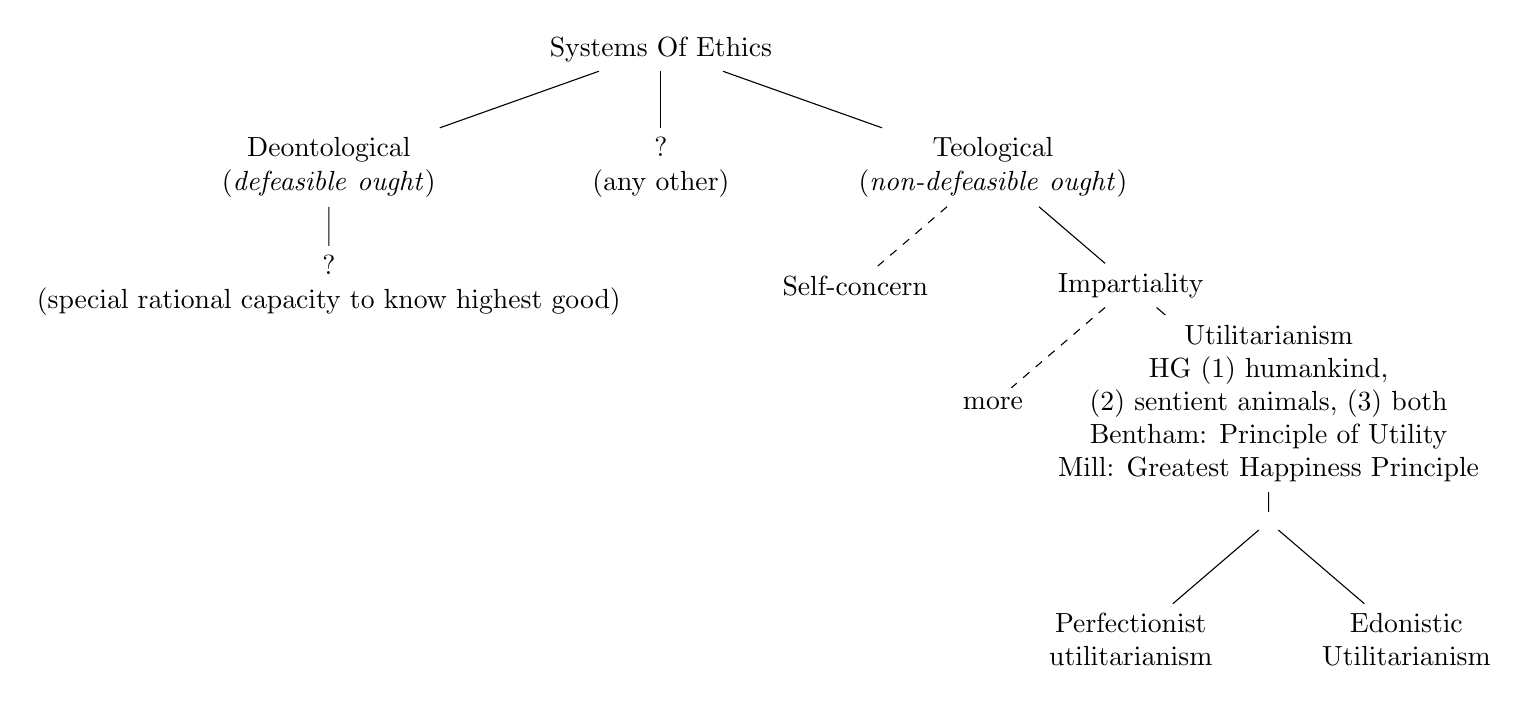
\begin{tikzpicture}[every node/.style={align=center},level 1/.style={sibling distance=12em},level 2/.style={sibling distance=35mm}, level 3/.style={sibling distance=30mm} level 4/.style={sibling distance=30mm}
]
\node {Systems Of Ethics}
    [sibling distance=6cm]
child { node {Deontological \\ (\textit{defeasible} \textit{ought})} 
child { node {? \\ (special rational capacity to know highest good)}}} % <- End Deontological
child { node {? \\ (any other)} }
child { node {Teological \\ (\textit{non-defeasible} \textit{ought})} child {node {Self-concern} \ed} child {node {Impartiality} child {node {more} \ed} 
child {node {Utilitarianism \\ HG (1) humankind, \\ (2) sentient animals, (3) both \\ Bentham: Principle of Utility \\ Mill: Greatest Happiness Principle}
child {node [] {} 
child {node {Perfectionist \\ utilitarianism} }
child {node {Edonistic \\ Utilitarianism}}}} }}
;
\end{tikzpicture}

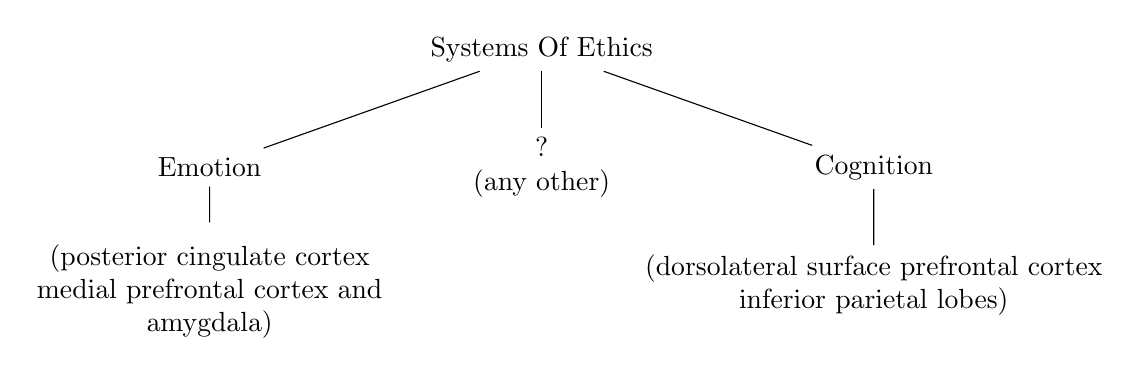
\begin{tikzpicture}[every node/.style={align=center},level 1/.style={sibling distance=12em},level 2/.style={sibling distance=35mm}, level 3/.style={sibling distance=15mm} level 4/.style={sibling distance=30mm}
]
\node {Systems Of Ethics}
[sibling distance=6cm]
child { node {Emotion} 
child { node { \\ (posterior cingulate cortex \\ medial prefrontal cortex and \\ amygdala)}}} % <- end emotion
child { node {? \\ (any other)} } % <- end any
child { node {Cognition} child{ node {(dorsolateral surface prefrontal cortex \\  inferior parietal lobes)}}} %<-end cognition
; %<-end node
\end{tikzpicture}

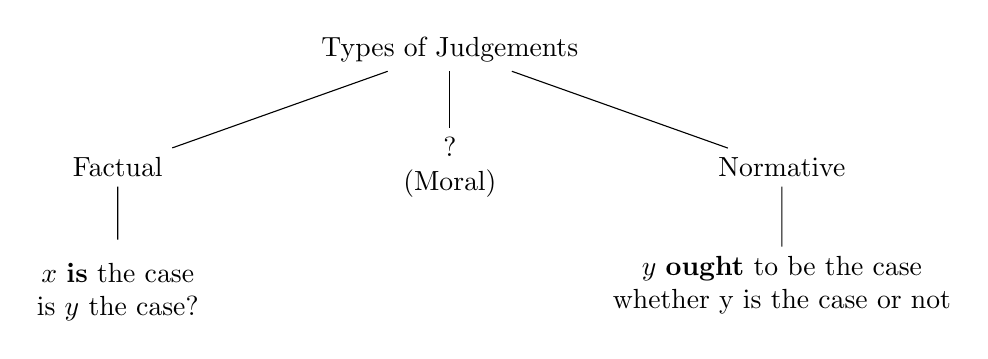
\begin{tikzpicture}[every node/.style={align=center},level 1/.style={sibling distance=12em},level 2/.style={sibling distance=35mm}, level 3/.style={sibling distance=15mm} level 4/.style={sibling distance=30mm}
]
\node {Types of Judgements}
[sibling distance=6cm]
child { node {Factual} 
    child { node { \\ \textit{$x$} \textbf{is} the case \\ is \textit{$y$} the case?}}} % <- end fact
child { node {? \\ (Moral)} } % <- end any
child { node {Normative} 
    child{ node {\textit{$y$} \textbf{ought} to be the case \\ whether y is the case or not}}} %<-end cognition
; %<-end node
\end{tikzpicture}

\end{document}